\subsection{Stationäres Streuproblem und Wirkungsquerschnitt}
	\begin{figure*} [h]
		\begin{center}
			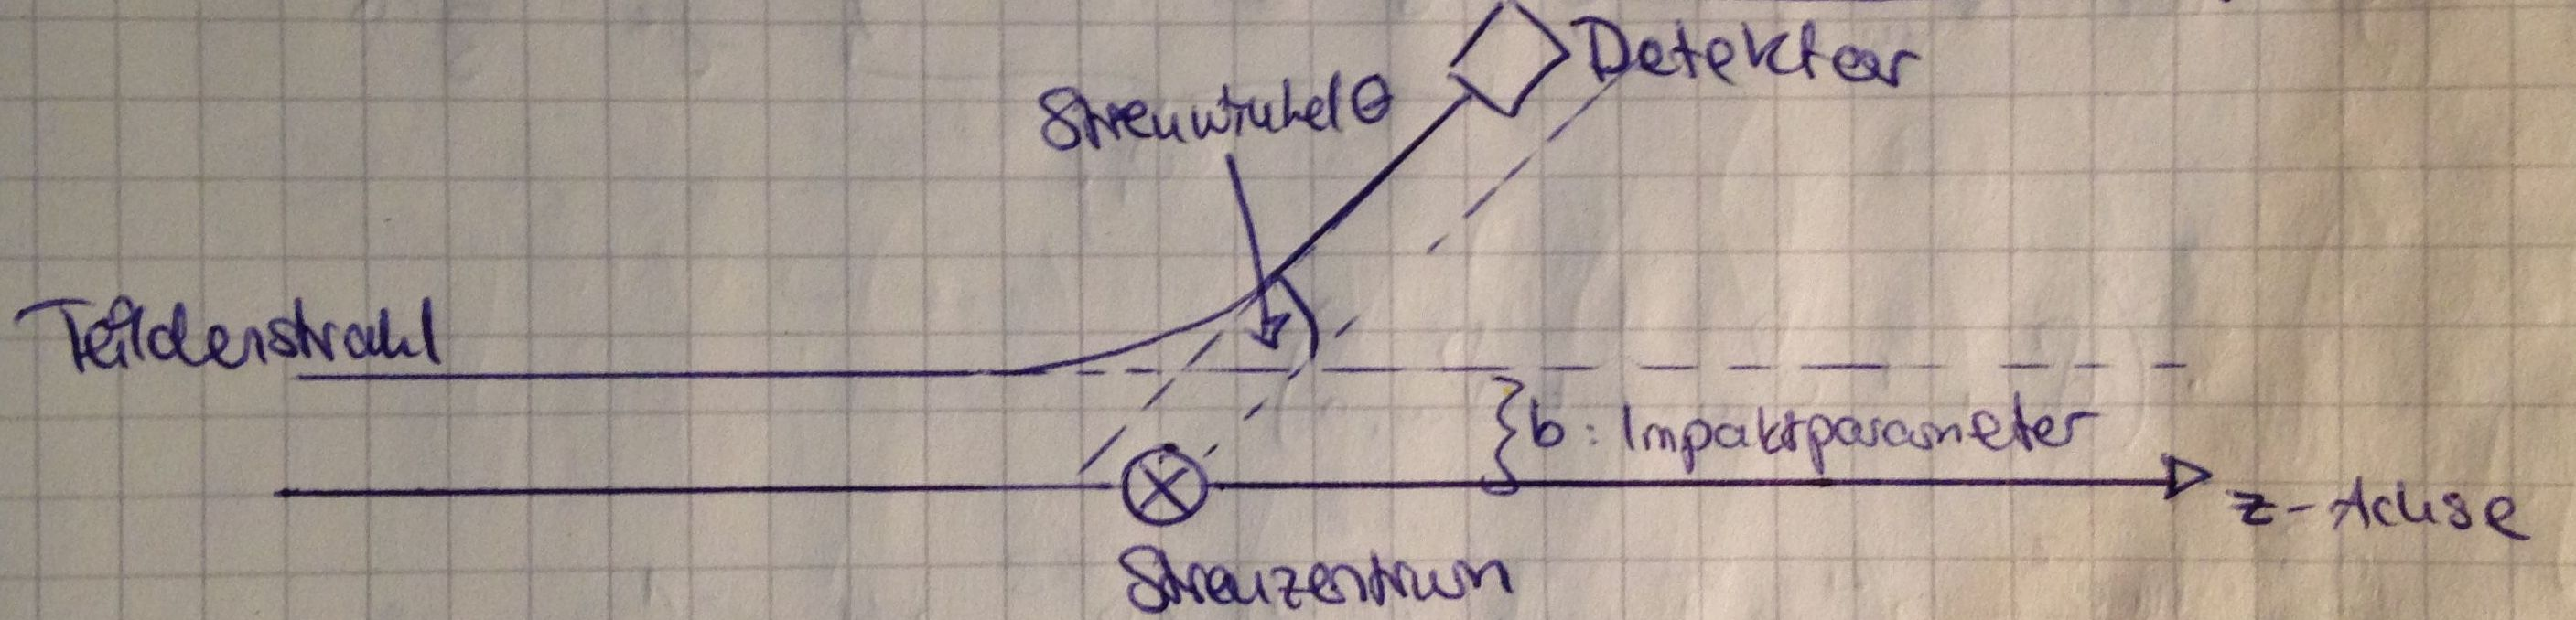
\includegraphics[width=12cm]{Stat_Streuproblem_Wirkungsquerschnitt}
		\end{center}
	\end{figure*}		
	Stromdichte des einlaufenden Teilchenstrahls: $\vec{j}_{ein}$
	\\

	\begin{minipage}[c]{0.3\textwidth}
				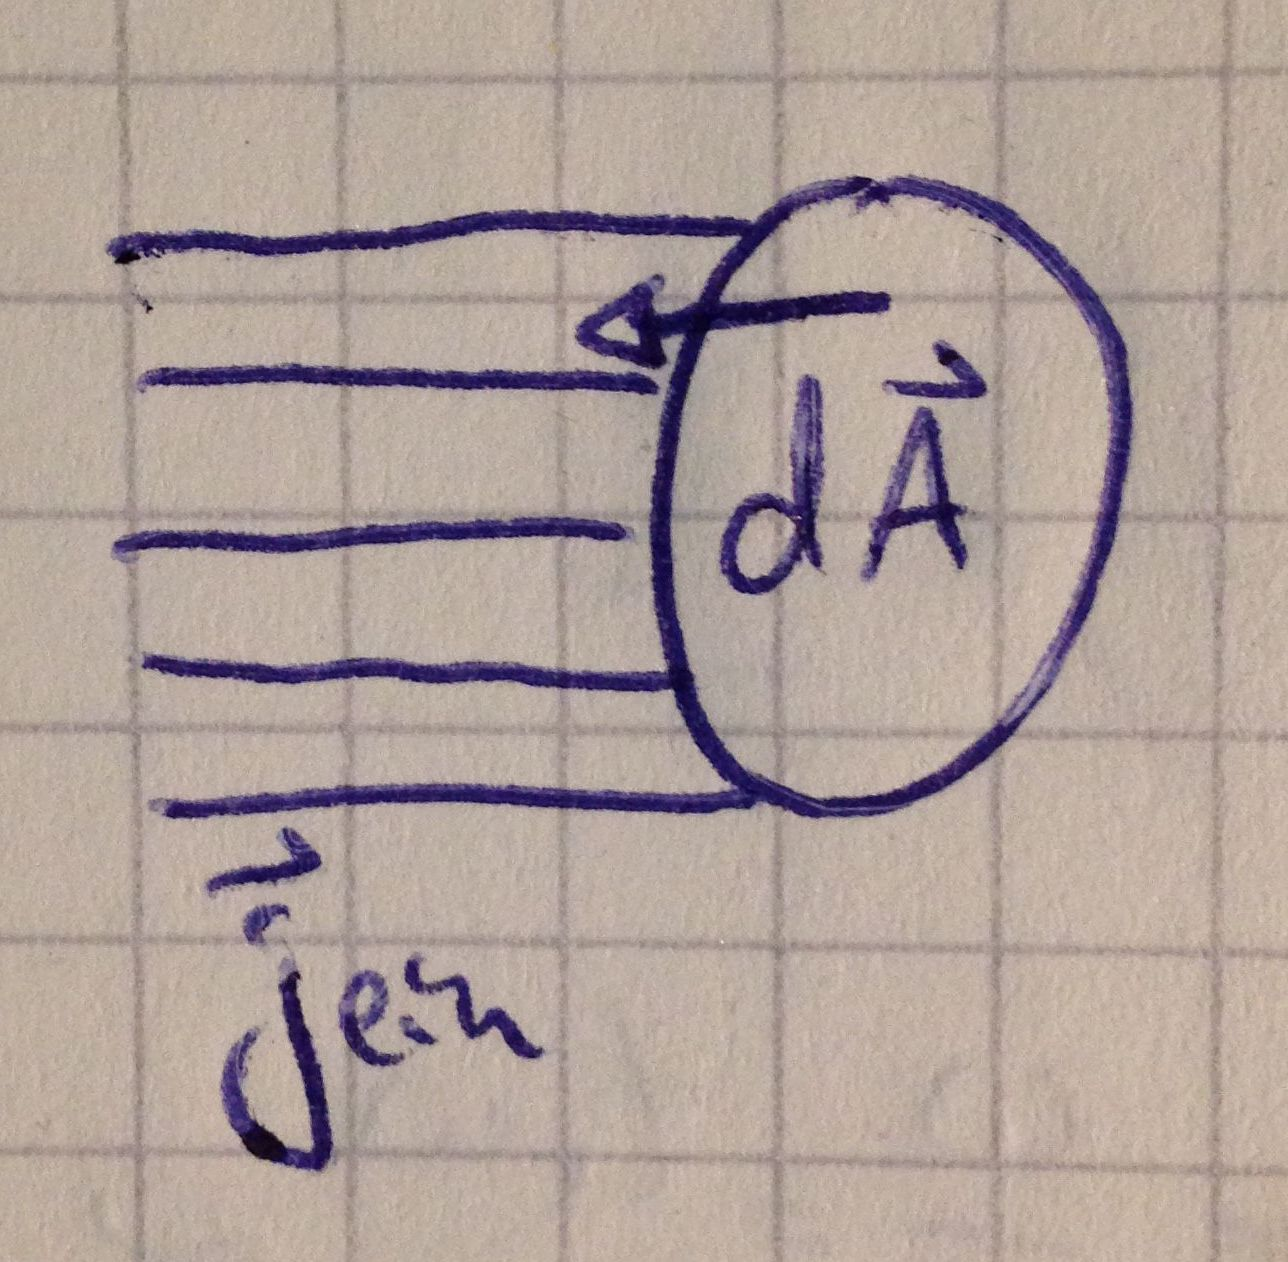
\includegraphics[width=\textwidth]{Stat_Streuproblem_Wirkungsquerschnitt2}
	\end{minipage}
	\hfill
	\begin{minipage}[c]{0.5\textwidth}
	Anzahl der Teilchen, die durch $\diff \vec{A}$ läuft:
		\begin{align*}
			\diff N &= 
			\underbrace{\vec{j}_{ein} \cdot \diff \vec{A}}_{\mathclap{\text{Strom}}}
			\cdot \diff t
		\end{align*}
	\end{minipage}
	\\	
	
	\begin{figure*} [h]
		\begin{center}
			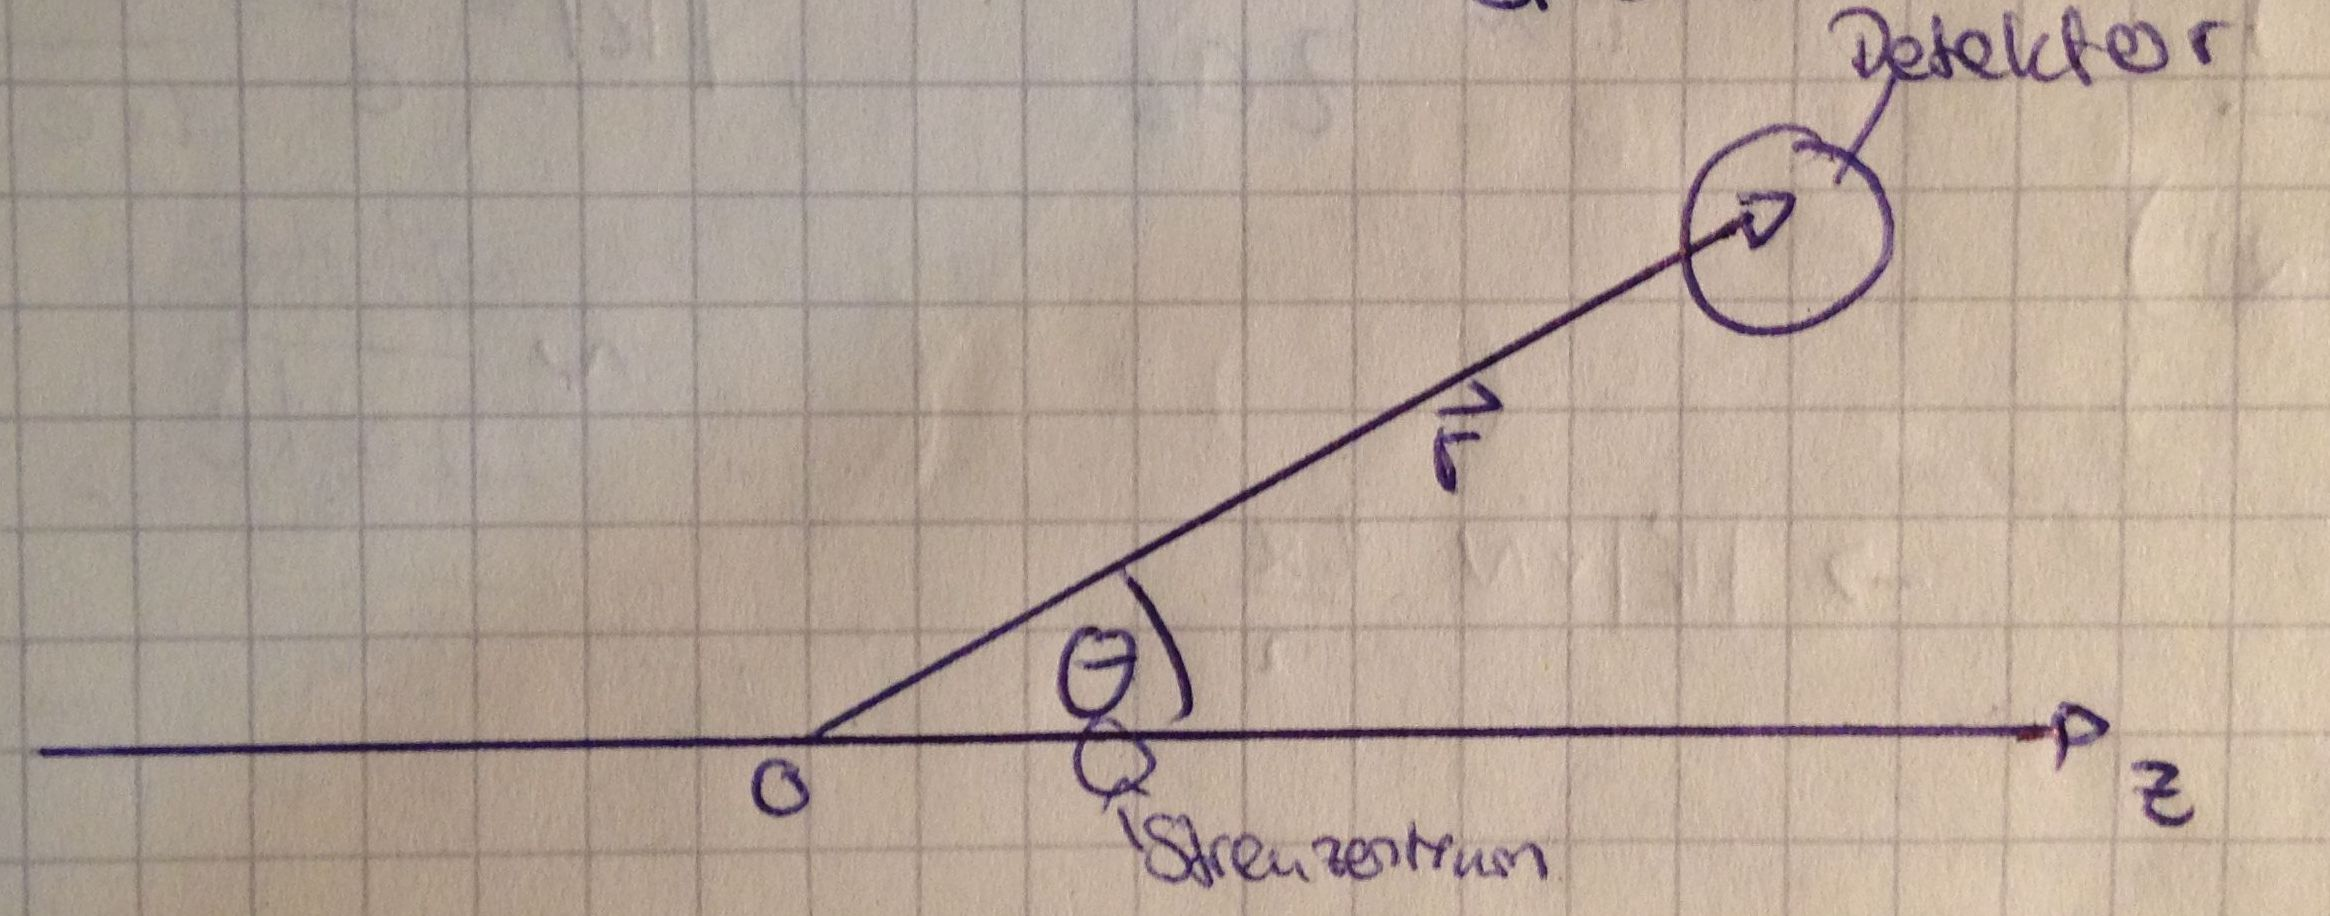
\includegraphics[width=10cm]{Stat_Streuproblem_Wirkungsquerschnitt3}
		\end{center}
	\end{figure*}
		\begin{align*}
			\diff A &= r^2 \diff \Omega = r^2 \diff \theta \sin \theta \diff \phi
		\end{align*}
	Differentieller Wirklungsquerschnitt $(r \rightarrow \infty)$
		\begin{empheq}[box=\boxed]{align*}
			\frac{\diff \sigma}{\diff \Omega} &=
			\frac{1}{|\vec{j}_{ein}|} \frac{\diff N}{\diff \Omega ~\diff t}
		\end{empheq}
	Homogener Strahl von Punktteilchen : $\vec{j} = \vec{v} \rho$ ($\rho$ ist Dichte)
		\begin{empheq}[box=\boxed]{align*}
			\frac{\diff \sigma}{\diff \Omega} &=
			\frac{|\vec{j}_{aus}(r, \theta, \phi)|}{|\vec{j}_{ein}|} ~r^2
		\end{empheq}
	$ \leadsto |\vec{j}_{aus}| \propto \frac{1}{r^2}$ (bei gleichen Detektorflächen $\diff A$)
	
	Totaler Wirkungsquerschnitt:
		\begin{align*}
			\sigma = \int \diff \Omega \frac{\diff \sigma}{\diff \Omega}
		\end{align*}
	Beispiel: Streuung an Scheibe der Fläche A:
	\\
	\begin{figure*} [h]
		\begin{center}
			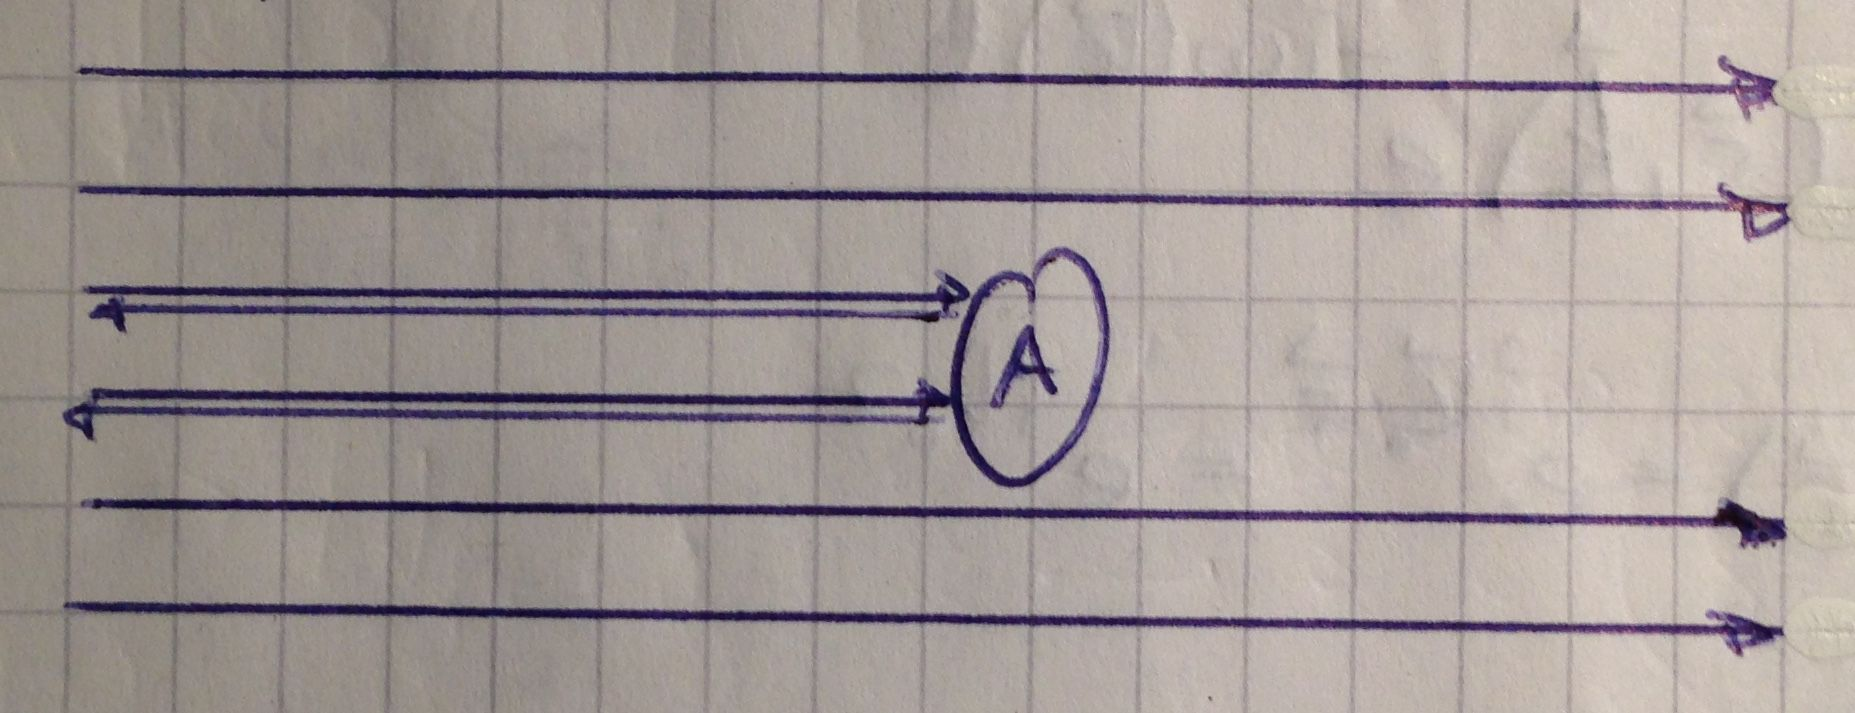
\includegraphics[width=10cm]{Stat_Streuproblem_Wirkungsquerschnitt4}
		\end{center}
	\end{figure*}
		\begin{align*}
			\sigma &= \int \diff \Omega \frac{\diff \sigma}{\diff \Omega}
			= \frac{1}{|\vec{j}_{ein}|} \int \diff \Omega \frac{\diff N}{\diff \Omega ~\diff t}\\
			&= \frac{1}{|j_{ein}|} \frac{\diff N}{\diff t} & &\frac{\diff N}{\diff t}: 
			\text{~Zahl gestreuter Teichen pro Zeit} \\
			&= \frac{1}{|j_ein|} \cdot |j_{ein}| \cdot A = A
		\end{align*}
	Schrödingergleichung: 
		\begin{equation*}
			i \hbar \frac{\partial \Psi (\vec{r}, t)}{\partial t} = H \Psi (\vec{r} , t) 
		\end{equation*}
	Einlaufendes Wellenpaket
	
	\begin{figure*} [h]
		\begin{center}
			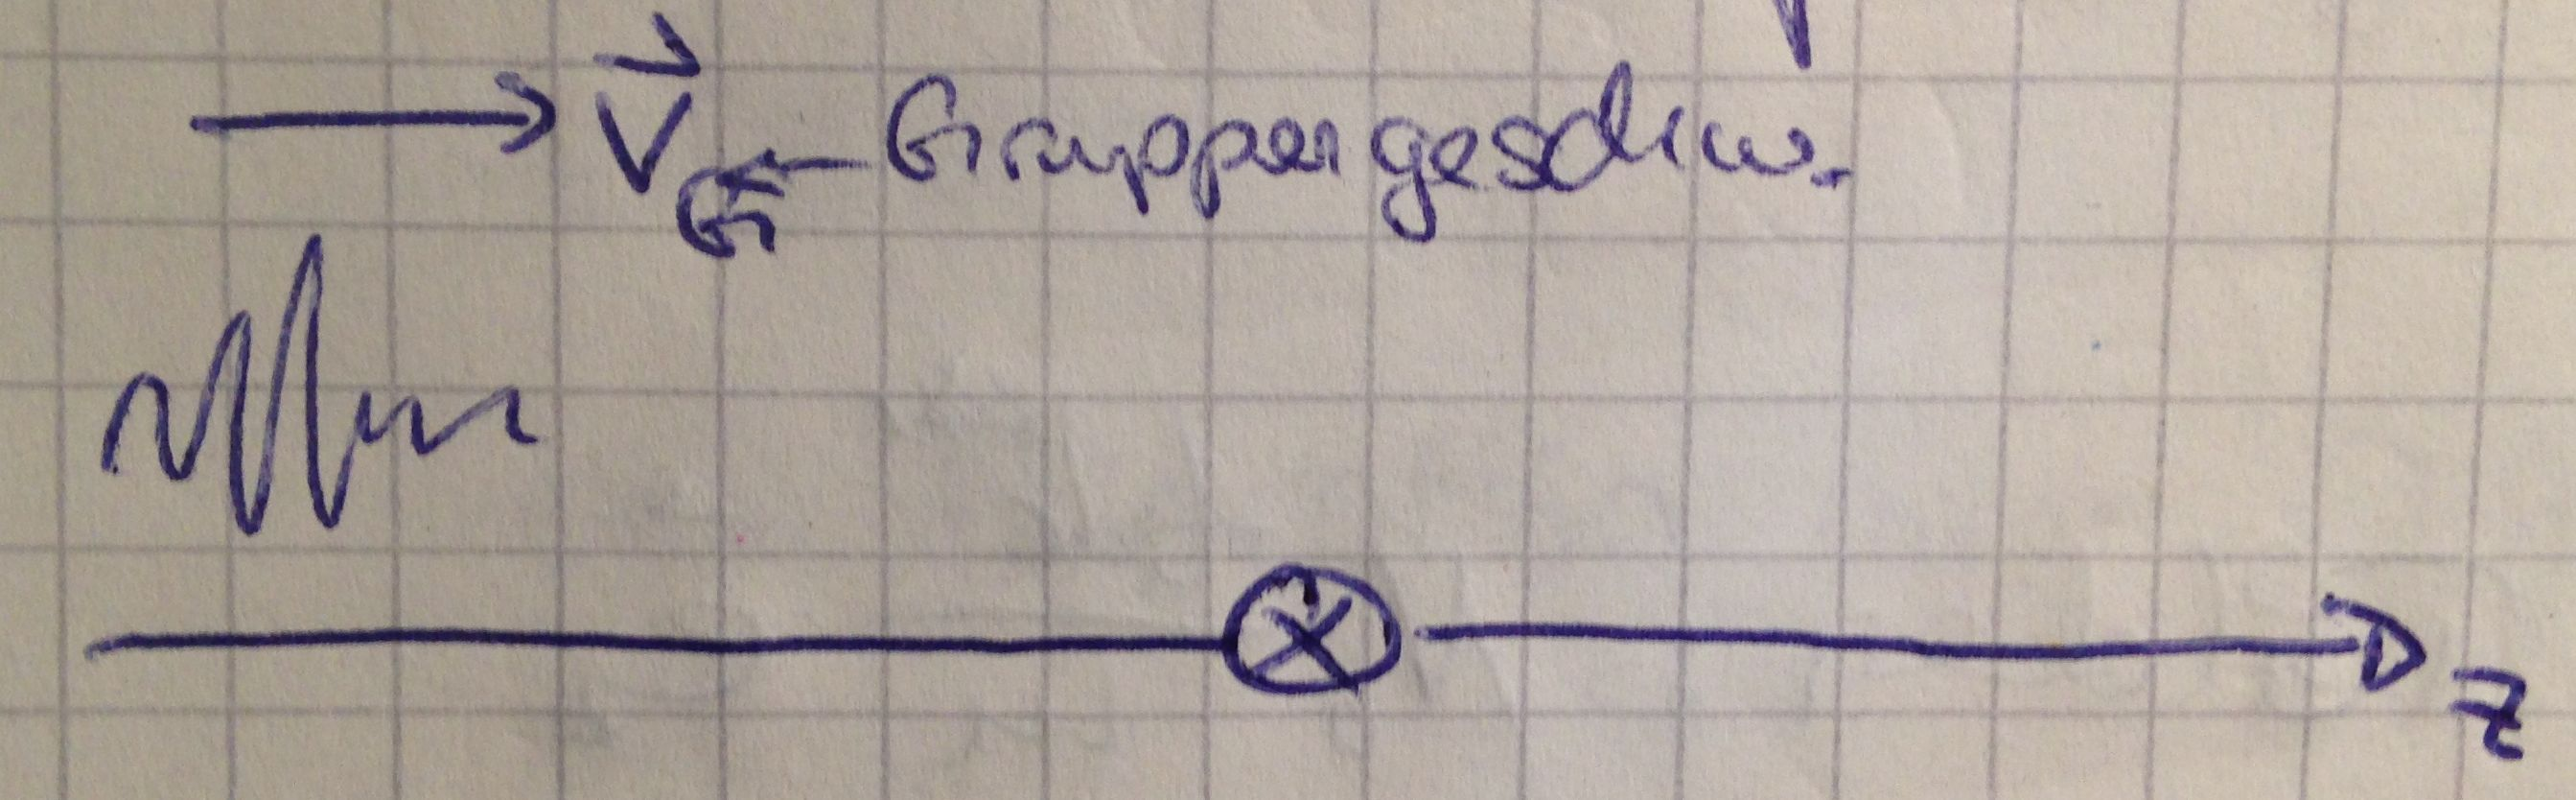
\includegraphics[width=10cm]{Stat_Streuproblem_Wirkungsquerschnitt5}
		\end{center}
	\end{figure*}
		\begin{equation*}
			\psi (\vec{r} , t) = 
			\int \frac{\diff^3 k}{(2 \pi)^3} A(\vec{k}) e^{i(\vec{k} \vec{r} - \omega(\vec{k}) t)}
		\end{equation*}
	Annahme:
		\begin{align*}
			v_G \ll c &\Rightarrow \omega(\vec{k}) = \frac{\hbar \vec{k}^2}{2 m} & &(V(\vec{r}) = 0 ~(\text{Potential}))
		\end{align*}
	Nebenbemerkung:
	
	Wir kennen bislang nur die nichtrelativistische Quantenmechanik. Die Streutheorie relativistischer Teilchen unterscheidet sich nicht \underline{wesentlich}.
	
	\begin{figure*} [h]
		\begin{center}
			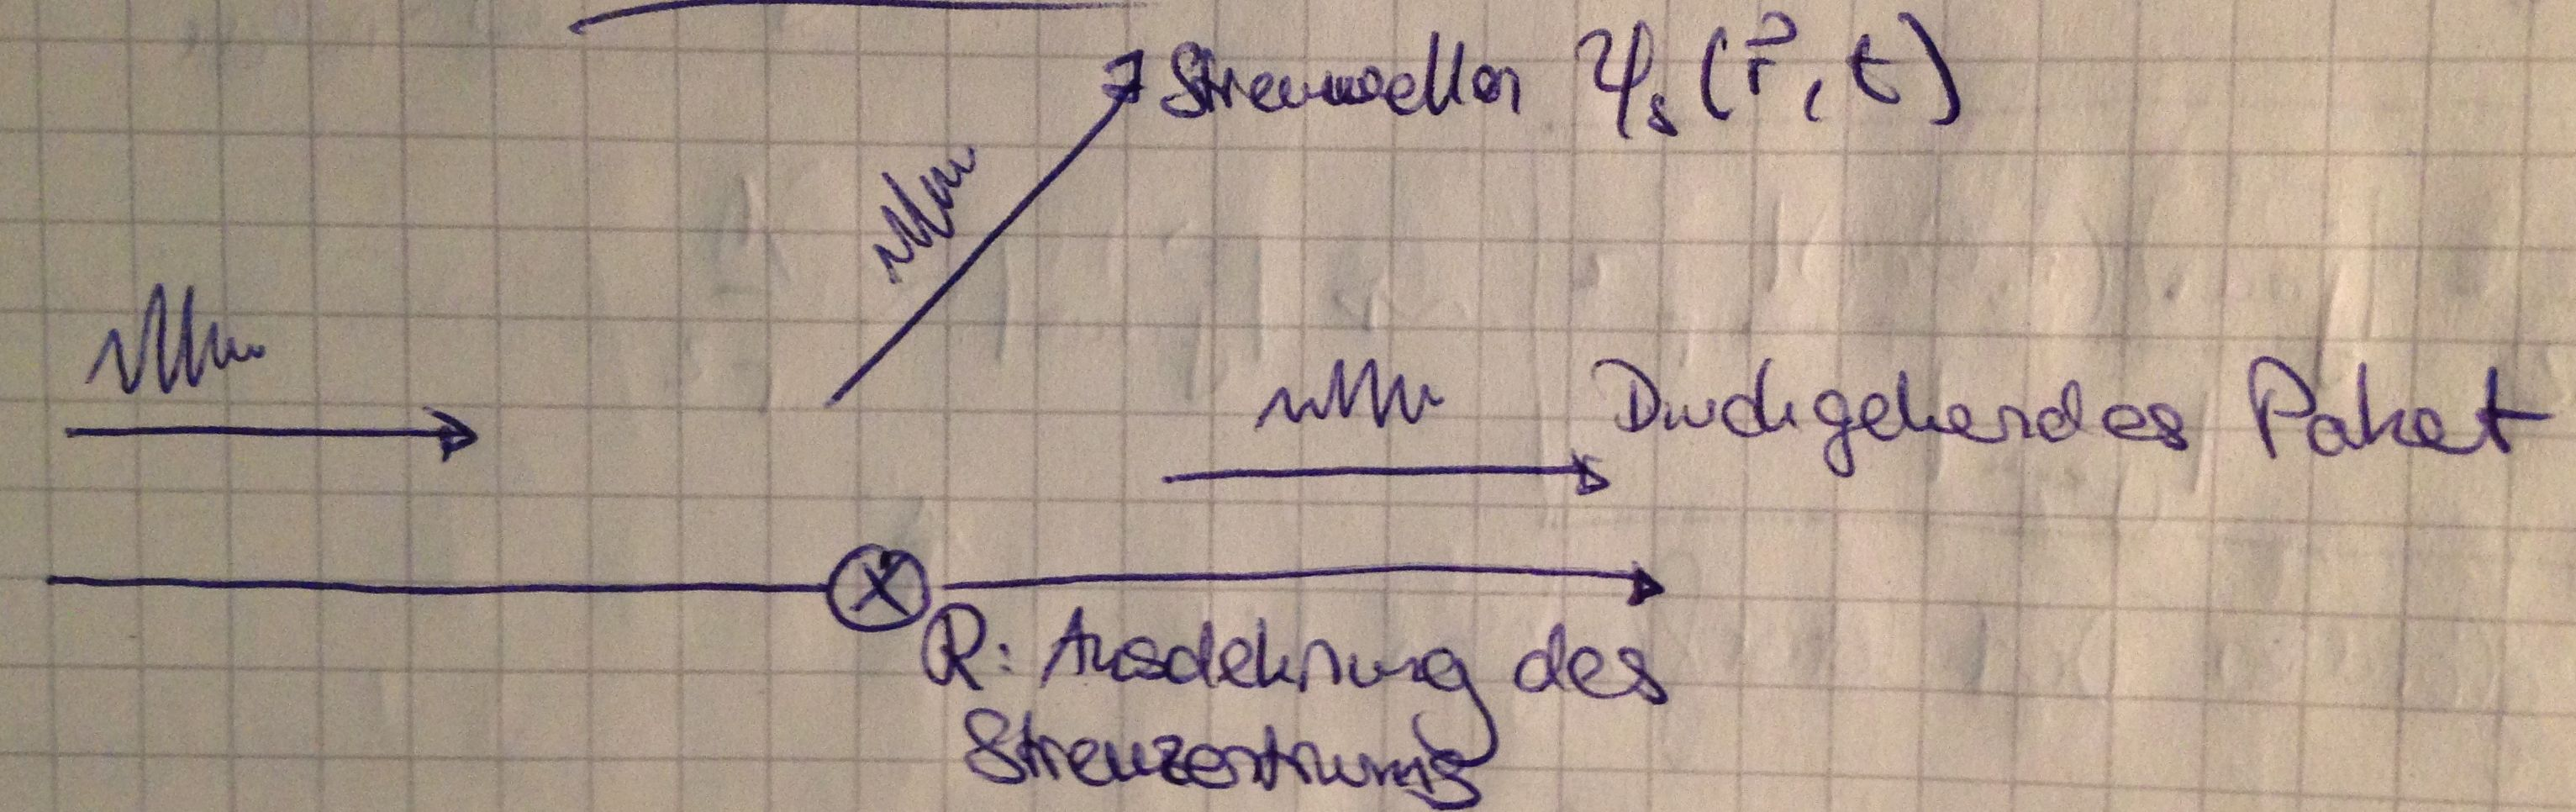
\includegraphics[width=12cm]{Stat_Streuproblem_Wirkungsquerschnitt6}
		\end{center}
	\end{figure*}
		\begin{align*}
			r &\gg R ,& r &\gg \lambda = \frac{2 \pi}{k} &\Rightarrow 
			&\text{gestreute Welle ist \underline{lokal} eine Kugelwelle} 
		\end{align*}
	Betrachte \underline{elastische} Streuung an Kugelsymmetrischem Störpotenial $V(r)$:
		\begin{align*}
			\psi_S (\vec{r}, t) &= 
			\int \frac{\diff^3 k}{(2 \pi)^3} A(\vec{k}) \phi_S (\vec{r}, \vec{k})
			e^{-i \omega (\vec{k}) t} \\
			&\text{Einfallender Strahl:} & \phi_0 (\vec{r}) &= e^{i \vec{k}_0 \vec{r}} = e^{i k_0 z}\\
			&\text{Gestreuter Strahl:} & \phi_S (\vec{r}) 
		\end{align*}
	Für $r \gg R$: Asymptotisch freie Wellen
	
	Einfallender Strahl:
		\begin{align*}
			\vec{p} &= \hbar k_0 \vec{e}_z ,& E &= \frac{\hbar^2 k_0}{2 m}\\
			-\frac{\hbar^2}{2 m} \vec{\nabla}^2 \phi_0 (\vec{r}) &= E \phi_0 (\vec{r})
		\end{align*}
	Wahrscheinlichkeitsstromdichte
		\begin{align*}
			\vec{j}_0 (\vec{r}, t) &=
			\frac{1}{2 m} 
			\left(\psi^* (\vec{r} , t) \vec{p} \psi (\vec{r}, t) - \psi (\vec{r}, t) \vec{p} \psi^* (\vec{r}, t)
			\right) \\
			&= \frac{\hbar k_0}{m} \vec{e}_z
		\end{align*}
	Nebenbemerkung: Teilchenstrom für $N_0$ Teilchen: $N_0 \frac{\hbar k}{m} \vec{e}_z$
	
	zu lösen ist:
		\begin{empheq}[box=\boxed]{align*}
			H \phi(\vec{r}) &= E \phi (\vec{r}) & &\text{für } E= \frac{\hbar k_0^2}{2 m} > 0\\
			H &= \frac{\vec{p}^2}{2 m} + V (r) & &V(r) \text{ begrenzt auf } r<R \\
			\phi (\vec{r}) &= e^{i k z} + \phi_S (\vec{r})
		\end{empheq}
	Ansatz:
		\begin{align*}
			\phi_S (\vec{r}) &\underset{r \rightarrow \infty}{\sim} f(\theta) \frac{e^{i k_0 r}}{r} &
			&\text{mit Streuamplitude } f(\theta)\\
			\vec{j} &= \frac{\hbar k_0}{m} \frac{|f(\theta)|^2}{r^2}
			\hat{e}_r (\theta , \phi) + \mathscr{O} \left(\frac{1}{r^3}\right)
		\end{align*}
		\begin{empheq}[box = \boxed]{align*}
			\frac{\diff \sigma}{\diff \Omega} = r^2 \frac{|\vec{j}_S|}{|\vec{j}_0|}
			= |f(\theta)|^2
		\end{empheq}
	Dieser Ansatz löst die Schrödingergleichung für $r \rightarrow \infty$ 
		\begin{align*}
			\underset{r \rightarrow \infty}{\lim} r V(r) &= 0 &
			&(\text{kein Coulomb-Potential})
		\end{align*}
	Streutheorie \marginpar{5.11.15}
	
	Kurze Wiederholung \marginpar{heute nicht Bali}
	
	\begin{figure*} [h]
		\begin{center}
			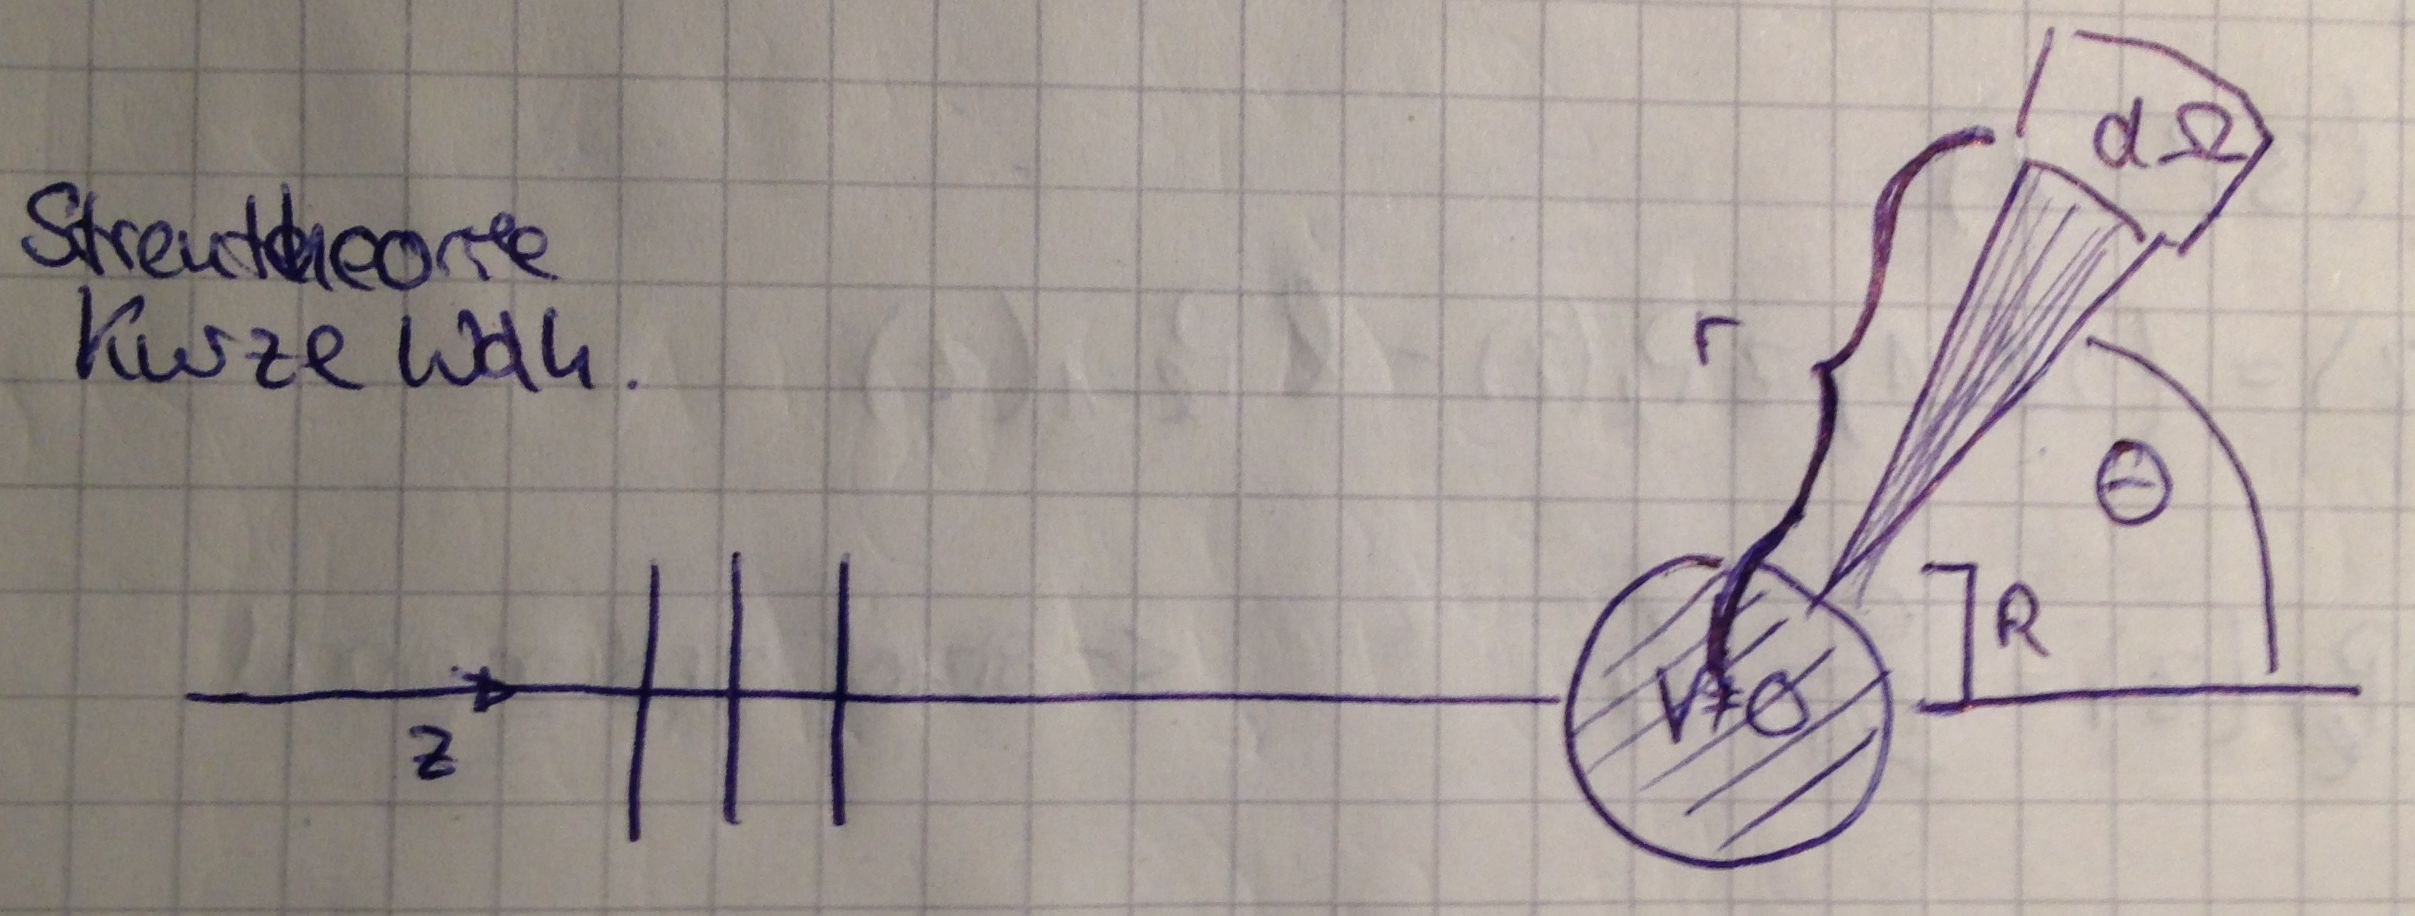
\includegraphics[width=10cm]{Stat_Streuproblem_Wirkungsquerschnitt7}
		\end{center}
	\end{figure*}
		\begin{align*}
			\diff A &= r^2 \diff \Omega ,& 
			\vec{j} &= \frac{\hbar}{2 m i} \left(\psi^* \vec{\nabla} \psi - \psi \vec{\nabla} \psi^* \right)
		\end{align*}
	$\diff N$ in diesem $\diff A$, in einem kleinen Zeitraum $\diff t$ \marginpar{??}
		\begin{align*}
			\frac{\diff \sigma}{\diff \Omega}
			&= \frac{|\vec{j}_{Streu}| ~\diff t ~ \diff A}{ |\vec{j}_{ein}| ~\diff t ~ \diff \Omega}
			=\frac{|\vec{j}_{Streu}| r^2}{|\vec{j}_{ein}|} :&
			&\text{hat Dimension Fläche}
		\end{align*}
	Annahmen:
		\begin{itemize}
			\item[-] 	Elastische Streuung, $\hbar k = \hbar k'$
			\item[-]	Stationäre Situation
			\item[-]	$V(\vec{r}) = V(|\vec{r}|)$ (Kugelsymmetrie)
			\item[-]	keine Absorption oder Emission
		\end{itemize}
	Wir wissen
		\begin{align*}
			\phi = \phi_0 + \phi_S = e^{i k z} + \phi_S
		\end{align*}
	$\phi$ ist im Bereich $r>R$ übereinstimmend mit Lösung der freien Schrödinger Gleichung.
		\begin{align*}
			\phi = \sum_{\ell = 0}^{\infty} R_\ell (r) 
			\underbrace{P_\ell (\cos \theta)}_{\mathclap{\sqrt{\frac{4 \pi}{2\ell+1}} 
					Y_{\ell 0}(\cos \theta)}} 
			& &[H, L_z] = 0 ~(\text{Drehimpulserhaltung})
		\end{align*}	
	\begin{figure*} [h]
		\begin{center}
			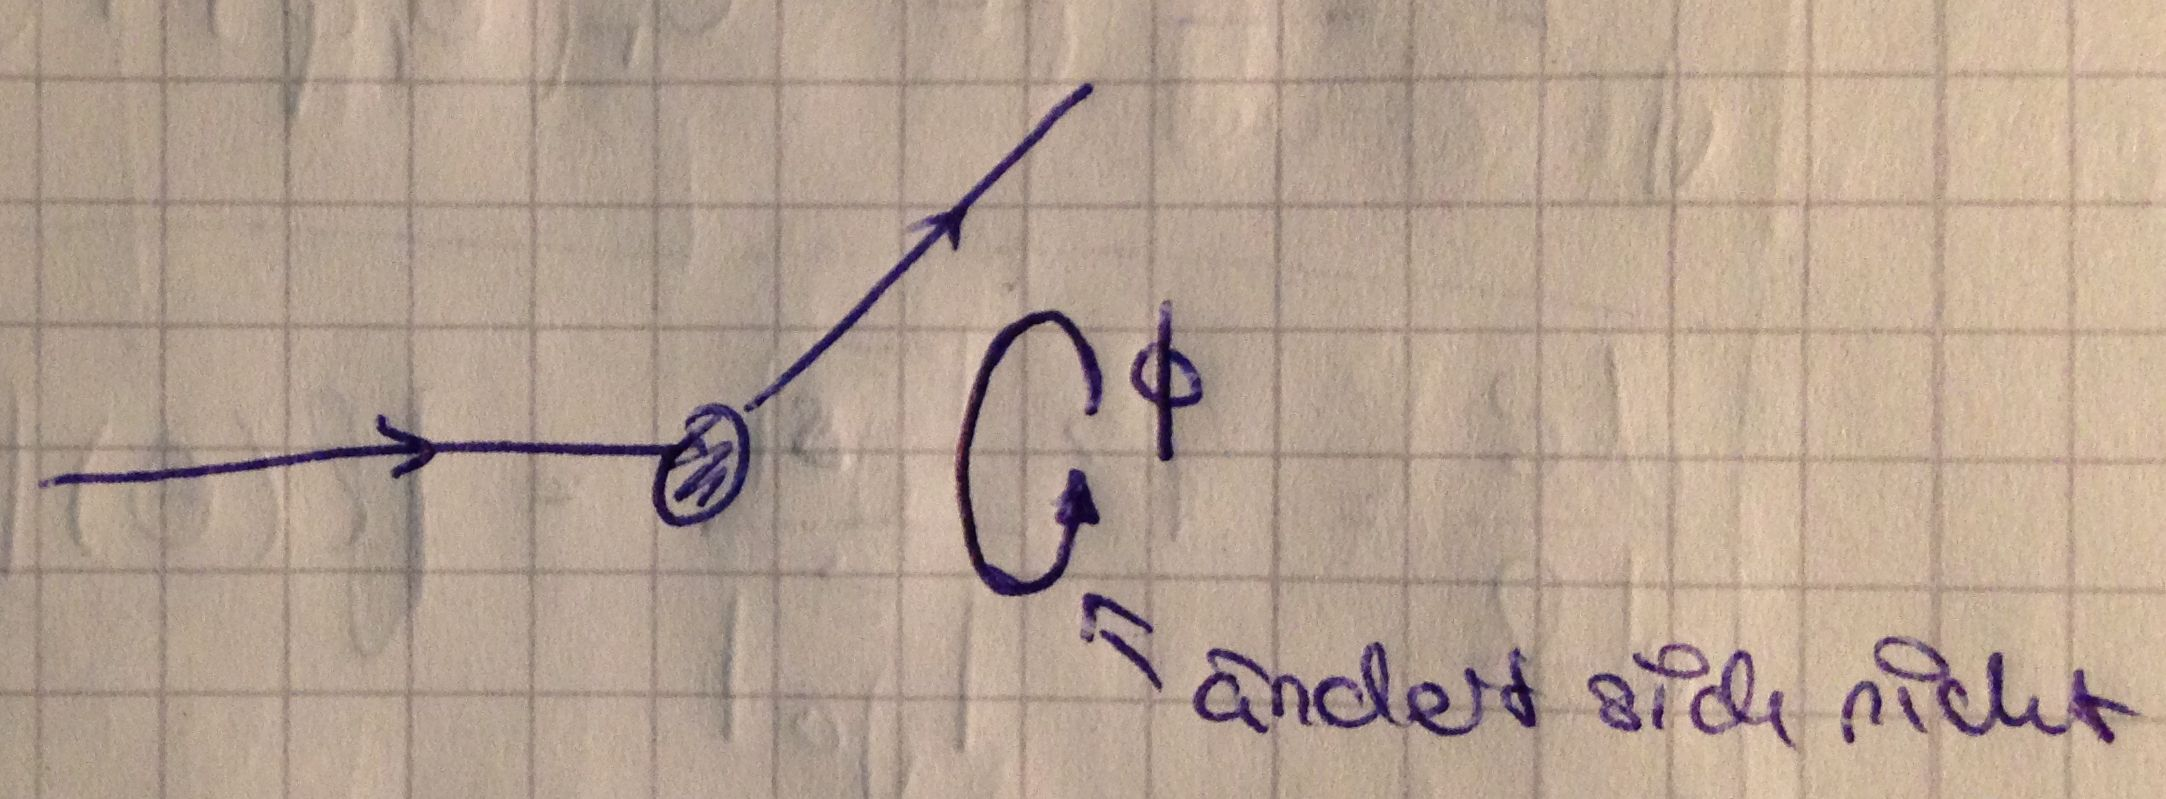
\includegraphics[width=10cm]{Stat_Streuproblem_Wirkungsquerschnitt8}
		\end{center}
	\end{figure*}
Symmetrisch bezüglich Drehachse
\FloatBarrier
	\underline{Legendre-Polynome $P_\ell (\cos \theta)$}
		\begin{align*}
			P_0 (\cos \theta) &= P_0 (z) = 1\\
			P_1 (z) &= z \\
			P_2 (z) &= \frac{1}{2} (3z^2-1) \\
			(\ell + 1) P_{\ell + 1} (z) &= (2 \ell + 1) z P_\ell (z) - \ell P_{\ell - 1} (z) \\
			\int_{-1}^{1} \diff z P_\ell (z) P_{\ell'} (z) &= 
			\frac{2}{2\ell + 1} \delta_{\ell \ell'} &
			&\leftarrow \text{ sind orthogonal}
		\end{align*}
		\begin{align*}
			-\frac{\hbar^2}{2m} \Delta \phi &= \frac{\hbar k^2}{2m} \phi \\
			\left( \frac{\partial^2}{\partial r^2} + \frac{2}{r} \frac{\partial}{\partial r} 
			- \frac{|\hat{L}|^2}{\hbar^2 r^2} + k^2
			\right) \phi &= 0 \\
			\sum_{\ell = 0}^{\infty} \underbrace{P_\ell (\cos \theta)}_{\mathclap{\text{orthogonal}}}
			\left( \frac{\partial^2}{\partial r^2} + \frac{2}{r} \frac{\partial}{\partial r} 
			- \frac{\ell(\ell+1)}{r^2} + k^2
			\right) R_\ell (r) &= 0
		\end{align*}
	$\Rightarrow$ Jeder Summand muss für sich verschwinden!
		\begin{align*}
			R_\ell &= \frac{u_\ell}{r} &\rightarrow &\text{ Ratialgleichung für } u_\ell \\
			\left( \frac{\partial^2}{\partial r^2} - \frac{\ell(\ell+1)}{r^2} + k^2
			\right) u(r) &= 0
		\end{align*}
	Beschränkung auf $r\gg R$ (wir können den Term $\frac{\ell(\ell+1)}{r^2}$ vernachlässigen)
		\begin{align*}
			\rightarrow u_\ell(r \gg R) &\rightarrow \text{ Kombination aus } \sin (kr) \text{ und } \cos(kr) \\
			u_\ell(r) &= c_\ell (k) \sin \left( kr - \frac{\ell \pi}{2} + \delta_\ell \right)
		\end{align*}
	Wobei $\delta_\ell$ die Streuphase ist. 
	
	Teile der Radialgleichung von $u_\ell$ durch $k^2$, $y=kr$ \marginpar{???}
		\begin{align*}
			\left( \frac{\diff^2}{\diff y^2} - \frac{\ell(\ell+1)}{y^2} + 1
			\right) u_\ell (y) &= 0 \\
			u_\ell^r &= y j_\ell (y) & & \text{ist reguläre Klasse (was auch immer das bedeutet)} \\
			&j_\ell (y) : & &\text{sphärische Besselfunktion} \\
			u_\ell^{ir} &= y n_\ell(y) & &\text{ist irreguläre Klasse}\\
			&n_\ell(y) : & &\text{sphärische Neumann-Funktionen}
		\end{align*}
		\begin{align*}
			j_0 &= \frac{\sin y}{y} ,& j_1 &= \frac{\sin y}{y^2}- \frac{\cos y}{y} \\
			n_0 &= -\frac{\cos y}{y} ,& n_1 &= -\frac{\cos y}{y^2} - \frac{\sin y}{y}
		\end{align*}
		\begin{align*}
			y ~j_\ell &= y^{\ell + 1} \left(-\frac{1}{y} \frac{\diff}{\diff y}\right)^\ell 
			\frac{\sin y}{y} &
			y ~n_\ell &= - y^{\ell+1} \left(-\frac{1}{y} \frac{\diff}{\diff y}\right)^\ell
			\frac{\cos y}{y}\\
			j_\ell(kr) &\overset{\text{große }kr}{\longrightarrow} 
			\frac{\sin(kr-\frac{\ell \pi}{2})}{kr} &
			n_\ell(kr) &\overset{\text{große }kr}{\longrightarrow} 
			- \frac{\cos(kr-\frac{\ell \pi}{2})}{kr} \\
			\phi_0 &= e^{ikz} = e^{ikr \cos \theta} =
		\end{align*}
		\begin{empheq}[box=\boxed]{align*}
			= \sum_{\ell = 0}^{\infty} (2\ell + 1) i^\ell j_\ell(kr) P_\ell (\cos \theta)
		\end{empheq}
	Für große $r$:
		\begin{align*}	
			\phi_S &= \phi - \phi_0 \\
			&= \sum_{\ell = 0}^{\infty} 
			\left[ \frac{c_\ell(kr)}{kr} \sin \left(kr-\frac{\ell \pi}{2} + \delta_\ell \right)
				-(2\ell +1)i^\ell \frac{\sin \left(kr-\frac{\ell \pi}{2}\right)}{kr}
			\right] P_\ell (\cos \theta)
		\end{align*}
	wobei $\delta_\ell \neq 0$ wegen $V \neq 0$.
	
	Diese Form enthält einlaufende und auslaufende Wellen. Wir wollen also nur $\frac{e^{+ikr}}{r}$ Terme behalten und $\frac{e^{-ikr}}{r}$ ist die Welle die vom Detektor zum Potential geht und diese soll sich wegheben $\rightarrow \delta_\ell$.
		\begin{align*}
			-c_\ell i^\ell e^{-i\delta_\ell} + (2 \ell + 1) i^{-2\ell} &= 0 &
			&(\text{ist nur erfüllt mit } e^{i\frac{\pi}{2}} = i^\ell) \\
			c_\ell &= i^{\ell} (2\ell + 1) e^{i \delta_\ell}\\
			\phi = \phi_0 + \phi_S &= e^{ikr \cos \theta} + f(\theta, k) \frac{e^{ikr}}{r}
		\end{align*}
	$f(\theta,k)$ ist die Streuamplitude.
		\begin{align*}
			f(\theta,k) &= \frac{1}{2ik} \sum_{\ell = 0}^{\infty} (2 \ell +1) P_\ell (\cos \theta) 
			\left(e^{2i\delta_\ell} - 1\right) & 
			&\text{ist } 0 \text{ für } \delta_\ell \rightarrow 0 \\
			\vec{j}_{\text{aus}} &= 
			\frac{\hbar}{2mi} \left(\phi_S^* \vec{\nabla} \phi_S
				- \phi_S \vec{\nabla} \phi_S^*
			\right) 
			= \frac{\hbar k}{m} \frac{|f(\theta, k)|^2}{r^2} \vec{e}_r
			+ \mathscr{O}\left(\frac{1}{r^3}\right) \\
			\vec{j}_{\text{ein}} &= \frac{\hbar k}{m} \vec{e}_r \\
			&\Rightarrow \frac{\diff \sigma}{\diff \Omega} = |f(\theta, k)|^2
		\end{align*}
	Der totale Wirkungsqerschnitt ist nun:
		\begin{align*}
			\sigma &= \int \diff \Omega \left(\frac{\diff \sigma}{\diff \Omega}\right)
			= \int \diff \Omega ~|f(\theta, k)|^2 
			= 2 \pi \int \diff \cos \theta ~|f(\theta, k)|^2 \\
			&= 2 \pi \sum_{\ell, \ell'} \int \diff \cos \theta 
			\frac{P_\ell (\cos \theta)~P_{\ell'} (\cos \theta)}{k^2} 
			\sin\delta_\ell ~\sin\delta_{\ell'} (2\ell+1) (2\ell' +1) \\
			&\left(
				\int_{-1}^{1} \diff \cos \theta ~ P_\ell P_{\ell'} = \frac{2}{2 \ell + 1} \delta_{\ell,\ell'}
			\right) \\
			&= \frac{4 \pi}{k^2} \sum_{\ell = 0}^{\infty}
			(2 \ell + 1) \sin^2 \delta_\ell
		\end{align*}
	Für kleine Energien nur $\delta_{\ell=0}$ wichtig
		\begin{align*}
			0 \lesssim \frac{4 \pi}{k^2} \\
			f(\theta, k) &= \sum_{\ell = 0}^{\infty} \frac{2 \ell + 1}{k} e^{i \delta_\ell}
			\sin \delta_\ell 
			\underbrace{P_\ell (\cos \theta)}_{\mathclap{P_\ell(\cos \theta = 1) = 1}} \\
			\mathrm{Im} f(\theta =0, k) &= \sum_\ell \frac{2 \ell + 1}{k} \sin^2 \delta_\ell
		\end{align*}
		\begin{empheq}[box=\boxed]{align*}
			0 = \frac{4 \pi}{k} 
			\underbrace{\mathrm{Im} f(\theta = 0, k)}_{\substack{\text{Imaginärteil der Vorwärtsamplitude}}}
		\end{empheq}
	Dies ist das optische Theorem.
	
	Behauptung: Bei kleinen Energien dominieren kleine $\ell$
	
	\begin{figure*} [h]
		\begin{center}
			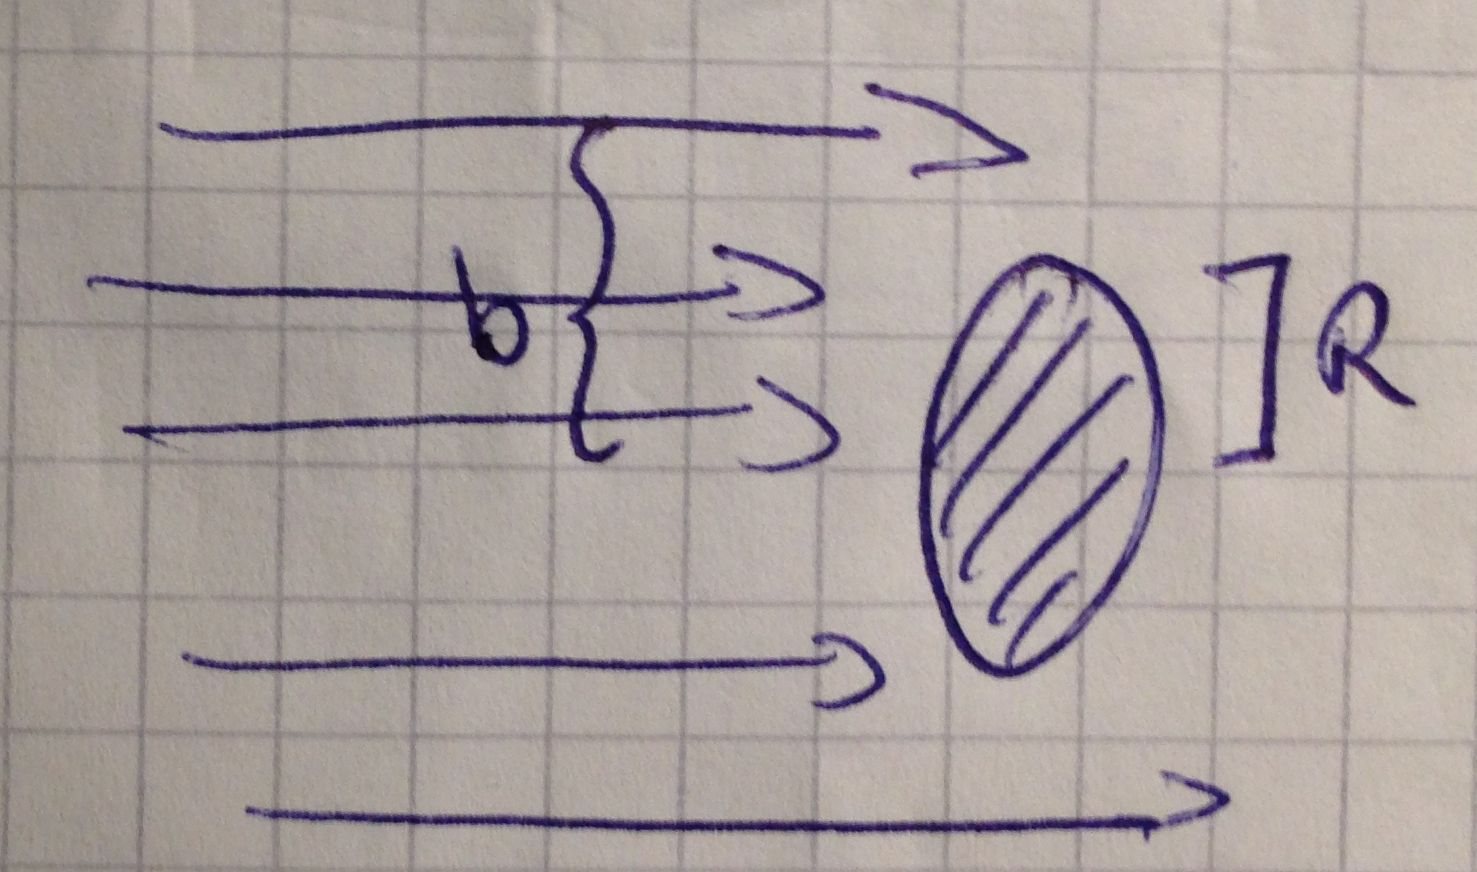
\includegraphics[width=8cm]{Stat_Streuproblem_Wirkungsquerschnitt9}
		\end{center}
	\end{figure*}
\FloatBarrier
	Wir haben den Stoßparameter $b$ und es gilt
		\begin{align*}
			L &= r \times p = \sqrt{2mE} ~b & &\text{ wenn } b > R \rightarrow \text{ kaum Streuung} \\
			|L| &\leq \sqrt{2 m E} ~R & &\text{ für Streuung}
		\end{align*}
	Interessante Observablen bei kleinen Energien:
	
	\underline{Streulänge} $a$ und ``effektive Reichweite $r_{\text{eff}}$''
		\begin{empheq}[box=\boxed]{align*}
			\ell = 0
		\end{empheq}
		\begin{align*}
			k \cot \delta_0 &= 
			-\frac{1}{a_0} + \frac{r_{\text{eff}}}{2} k^2 + \mathscr{O}(k^4) 
			& &a_0 \text{ ist S-Wellen Streulänge} \\
			\text{Für } k &\rightarrow 0 \\
			0 &\rightarrow 4\pi a_0^2
		\end{align*}